\documentclass[runningheads]{llncs}
\usepackage{amssymb,booktabs,graphicx,xcolor,hyperref,array}
\usepackage{float}
\usepackage{tikz}
\usetikzlibrary{arrows.meta,positioning,fit,calc,backgrounds}
\usepackage{enumitem}
\setlist{nosep,leftmargin=2em}
\graphicspath{{figures/}}
\hypersetup{colorlinks=true,linkcolor=blue,urlcolor=blue,citecolor=blue,
  hypertexnames=false}
\renewcommand{\topfraction}{0.92}
\renewcommand{\bottomfraction}{0.88}
\renewcommand{\textfraction}{0.08}
\renewcommand{\floatpagefraction}{0.72}
\setlength{\textfloatsep}{12pt plus 3pt minus 3pt}
\setlength{\floatsep}{10pt plus 3pt minus 3pt}
\makeatletter
\setlength{\@fptop}{0pt}
\setlength{\@fpsep}{12pt}
\setlength{\@fpbot}{0pt plus 1fil}
\makeatother
\setlength{\emergencystretch}{2em}

\newcommand{\method}{M1}
\newcommand{\full}{FullSchema}
\newcommand{\schemarag}{SchemaRAG}

\title{Budget-Aware Dynamic Schema Adaptation for Efficient LLM-Based Information Extraction}
\titlerunning{Budget-Aware Dynamic Schema Adaptation}
\author{Hongjian Hu \and Letong Wang}
\authorrunning{Hu, H. \and Wang, L.}
\institute{School of Information Science and Technology,\\ Northwest University, Xi'an 710127, China}

\begin{document}
\catcode`\`=\active
\def`#1`{\texttt{\detokenize{#1}}}
\maketitle

\begin{abstract}
\begin{sloppypar}
 Cultural heritage records are heterogeneous in information density and in the fields that can be extracted reliably. Sending a full Schema to every record therefore introduces irrelevant field load for low-information records. We investigate whether model-assisted silver supervision generated by full-Schema extraction can support pre-call, record-level field selection, and whether field-value priors and estimated field costs can be incorporated into a budget-constrained dynamic Schema. We evaluate pruning cost by field-selection completeness rather than factual correctness of field values: on the 476-record shared-success subset of 500 model-assisted evaluation-reference records, `budget-200` covers 83.03\% of non-empty reference fields, with a 16.97\% selection-stage omission rate. After training on 100 silver records, a 2,000-record development-distribution workload shows that, under Qwen3-8B-AWQ~\cite{yang2025qwen3} service and a single-process bounded-queue configuration, `budget-200` uses fewer total tokens, has a shorter online pipeline time, and achieves higher effective throughput than the full Schema. Additional diagnostics indicate that token reduction is mainly attributable to fewer selected fields, while the current weighted ranking is not consistently better than equal, frequency-based, or simple Top-$k$ alternatives. These conclusions are bounded to the present data, model service, and single-process setting.
\end{sloppypar}
\end{abstract}

\keywords{Cultural heritage extraction \and Dynamic Schema \and Large language models \and Budget constraints \and Data preprocessing \and Online throughput}

\section{Introduction}

Cultural heritage databases accumulate records from many sources whose key names, description length, information density, and extractable fields vary widely. Sending the full Schema with every record simplifies invocation but attaches many irrelevant field definitions to low-information records, inflating input tokens, output tokens, and online inference time. In large-scale preprocessing this fixed Schema load can become a bottleneck; we make no end-to-end empirical claim for workloads of hundreds of thousands of records.

LLM-based structured extraction and retrieval-augmented studies show that models can populate a supplied Schema and narrow candidate fields from the input. Yet selecting too few fields risks omitting long-tail information, while selecting too many reintroduces Schema load. For cultural heritage records without large-scale human field annotations, it remains unclear whether the modest model-assisted silver supervision produced by full-Schema extraction provides sufficient signal for pre-call field pruning. We therefore ask whether record-level field selection can preserve high reference-field coverage and reduce runtime while raising effective throughput in an end-to-end pipeline that includes queuing, requests, retries, and result writing.

To answer this, we formulate record-level field selection as budget optimization: sparse textual features predict field presence and output length, and a budgeted selector combines field value, estimated cost, and mandatory-field constraints into a dynamic Schema. We use full-Schema extraction as the reference behavior and compare it with fixed Top-$k$ embedding-based field retrieval. The budget is the estimated capacity of field combination, not an API-token or monetary-cost cap; coverage judges only the selected field set, not the factual correctness of field values. We construct no human Gold, and all conclusions are bounded by the present data, model service, Prompts, and single-process pipeline.

\section{Related Work}

ChatSchema~\cite{chatschema}, UIE~\cite{uie}, and InstructUIE~\cite{instructuie} extract against a supplied Schema. \schemarag{}~\cite{schemarag} retrieves a fixed Top-$k$ field set by record--metadata similarity, whereas PARSE~\cite{parse} and Schema-adaptable Knowledge Graph Construction~\cite{adakgc} address JSON contracts and global Schema evolution. These approaches do not jointly address pre-call, record-level selection of relatively stable candidate fields, an auditable field-capacity constraint, and online measurement of the load--completeness trade-off. We combine silver-label behavior scores, field value, estimated cost, and budgeted selection.

Doctopus~\cite{doctopus}, FrugalGPT~\cite{frugalgpt}, and LLMLingua~\cite{llmlingua} control plans, models, or textual tokens, not Schema-field selection or reference-field omission against online metrics. Our \schemarag{} is an external fixed Top-$k$ adaptation based on its public description, not the official implementation. PagedAttention~\cite{pagedattention} optimizes the KV cache; our single-process Runner measures only request-load effects of field pruning. Huang et al.~\cite{huang2023} provide digital-heritage context, not cross-dataset or production-scale evidence.

\section{Method}

Let $r$ denote a raw record, $F$ the candidate-field set, and $S_r\subseteq F$ the selected fields. For field $f$, the selector predicts a presence score $p(r,f)$ and an output-token count $\hat{o}(r,f)$. The field-value weight $w_f$ is an auditable task heuristic, not a weight learned as optimal from the present data, and $d_f$ is the field-definition cost. Dynamic selection is written as

\begin{equation}
 u(r,f)=p(r,f)w_f,
 \qquad c(r,f)=d_f+\hat{o}(r,f),
 \label{eq:utility-cost}
\end{equation}
\begin{equation}
 \max_{S_r}\sum_{f\in S_r}u(r,f),
  \quad \mathrm{s.t.}\quad \sum_{f\in S_r}c(r,f)\leq B.
\end{equation}

Here $B$ is the estimated field-cost capacity for the selection stage, not an end-to-end token or monetary-cost limit for the LLM call. Final tokens also include raw text, fixed Prompt, actual output, and retry consumption.

As shown in Fig.~\ref{fig:overall-framework}, the offline stage trains \method{} from \full{} silver labels. The online stage serializes each record, predicts and selects fields under the budget, constructs a dynamic Schema, invokes the LLM, and writes the result.

\begin{figure}[!ht]
\centering
\resizebox{\linewidth}{!}{%
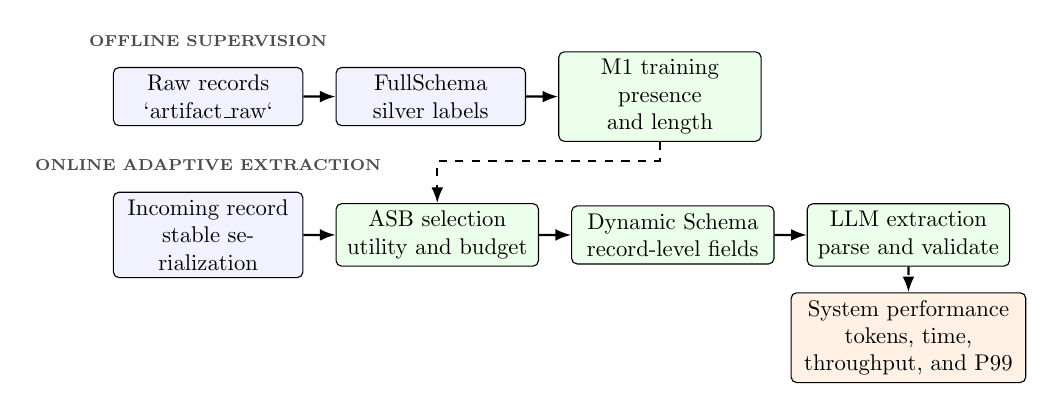
\begin{tikzpicture}[scale=0.82,transform shape,node distance=4mm and 5mm,
 data/.style={draw, rounded corners=2pt, align=center, minimum height=7mm, text width=27mm, fill=blue!5},
 process/.style={draw, rounded corners=2pt, align=center, minimum height=7mm, text width=29mm, fill=green!8},
 eval/.style={draw, rounded corners=2pt, align=center, minimum height=7mm, text width=34mm, fill=orange!10},
 stage/.style={font=\bfseries\scriptsize, text=black!70},
 arrow/.style={-{Latex[length=2mm]}, thick},
 dependency/.style={-{Latex[length=2mm]}, thick, dashed},
 evalarrow/.style={-{Latex[length=2mm]}, thick, dashed}]
\node[stage] (offline-title) {OFFLINE SUPERVISION};
\node[data, below=2mm of offline-title] (raw) {Raw records\\`artifact\_raw`};
\node[data, right=of raw] (silver) {\full{}\\silver labels};
\node[process, right=of silver] (train) {\method{} training\\presence and length};
\draw[arrow] (raw) -- (silver);
\draw[arrow] (silver) -- (train);
\node[stage, below=4mm of raw] (online-title) {ONLINE ADAPTIVE EXTRACTION};
\node[data, below=2mm of online-title] (record) {Incoming record\\stable serialization};
\node[process, right=of record] (select) {ASB selection\\utility and budget};
\node[process, right=of select] (schema) {Dynamic Schema\\record-level fields};
\node[process, right=of schema] (llm) {LLM extraction\\parse and validate};
\draw[dependency] (train.south) -- ++(0,-3mm) -| (select.north);
\draw[arrow] (record) -- (select);
\draw[arrow] (select) -- (schema);
\draw[arrow] (schema) -- (llm);
\node[eval, below=4mm of llm] (performance) {System performance\\tokens, time, throughput, and P99};
\draw[evalarrow] (llm.south) -- (performance.north);
\end{tikzpicture}%
}
\caption{Overall study design. Raw records construct \full{} silver-label supervision for \method{} training. The online path applies ASB selection before dynamic-Schema extraction. Evaluation reports model-assisted reference-field coverage and system performance; the reference is not independent human factual Gold.}\label{fig:overall-framework}
\end{figure}

\subsection{Data Representation and Silver Supervision}

The project database aligns \texttt{artifact\allowbreak\_raw} with \texttt{artifact\allowbreak\_extract} through `artifact_id`, yielding 6,763 records split into 5,410 training, 677 validation, and 676 test records. We consider 18 predefined target fields rather than arbitrary JSON keys; `artifact_id` is used only for joins, splitting, and result pairing. Record-type proportions in the performance workload differ from the source database by at most about 1.4 percentage points, and raw records usually contain only five non-empty fields; the results therefore do not claim coverage of all source distributions. A character 3-gram Jaccard scan (threshold 0.6) found 1,101 near-duplicate pairs and 111 clusters with a maximum size of 50; these structures and the 132 type--period proxy groups were retained to reflect the target distribution, without claiming independent generalization across templates or sources.

The candidate Schema contains the same 18 fields. `name` and `category` are mandatory, `desc` uses a constant presence prediction, and the selector chooses the remaining fields per record. Several long-tail fields have silver non-empty rates below 2\%. Field weights are auditable task settings rather than learned optimal weights; complete definitions are supplied with the manuscript materials. \full{} uses all fields, whereas the dynamic Schema selects a subset $S_r\subseteq F$.

`artifact_extract` is a model-assisted silver reference produced by the \full{} process, not human ground truth: a non-empty output for field $f$ gives `present=1`, and the `cl100k_base` token count of a non-empty value gives the length label. \method{} therefore learns \full{} output behavior rather than independently verified factual truth.

\subsection{Field Predictor and Dynamic Selection}
\subsubsection{Field Predictor Based on Sparse Text Features}

Raw JSON keys, values, and description text are stably serialized into a record-level text representation (`record_text`). The label $y_f(r)$ indicates whether the \full{} silver output for field $f$ is non-empty; the encoded length of a non-empty value supplies output-length supervision. Training, validation, and test sets are separated by `artifact_id`, and validation is used only for threshold calibration. Each field uses an independent balanced logistic-regression classifier. The length branch fits $\log(1+o_f(r))$ and falls back to the median when positive examples are insufficient.

\method{} concatenates character-level and word-level TF--IDF features and outputs $p(r,f)$ and $\hat{o}(r,f)$; the character model is used only as a baseline. \textsc{M2} separately trains the two feature types and linearly fuses their probabilities, solely as an offline ablation. The vocabulary is fitted only on the training subset. Training sizes are $n\in\{50,100,250,500,1000,2500,5410\}$, using nested prefixes and seeds 42--46. `name`, `category`, and `desc` use constant predictions; insufficient positive examples for long-tail fields limit macro-averaged performance.

\begin{sloppypar}
\setlength{\emergencystretch}{4em}
In a test replay of 100 startup samples, the character baseline achieved macro/micro Presence F1 and length MAE of $0.5187/0.9126/4.8046$. The corresponding values were $0.5088/0.9343/4.7615$ for \method{} and $0.5083/0.9341/4.7615$ for \textsc{M2}. \method{} provided only slight improvements in micro averaging and length error, while \textsc{M2} provided no additional benefit. Detailed per-field results and intervals from 35 offline runs are supplied with the manuscript materials.
\end{sloppypar}

\begin{sloppypar}
Online, \method{} does not generate field values. The predictions are used with the mandatory-field constraint and a 0--1 knapsack to form $S_r$. Actual tokens are recorded from API calls.
\end{sloppypar}

\begin{figure}[htbp]
\centering
\resizebox{\linewidth}{!}{%
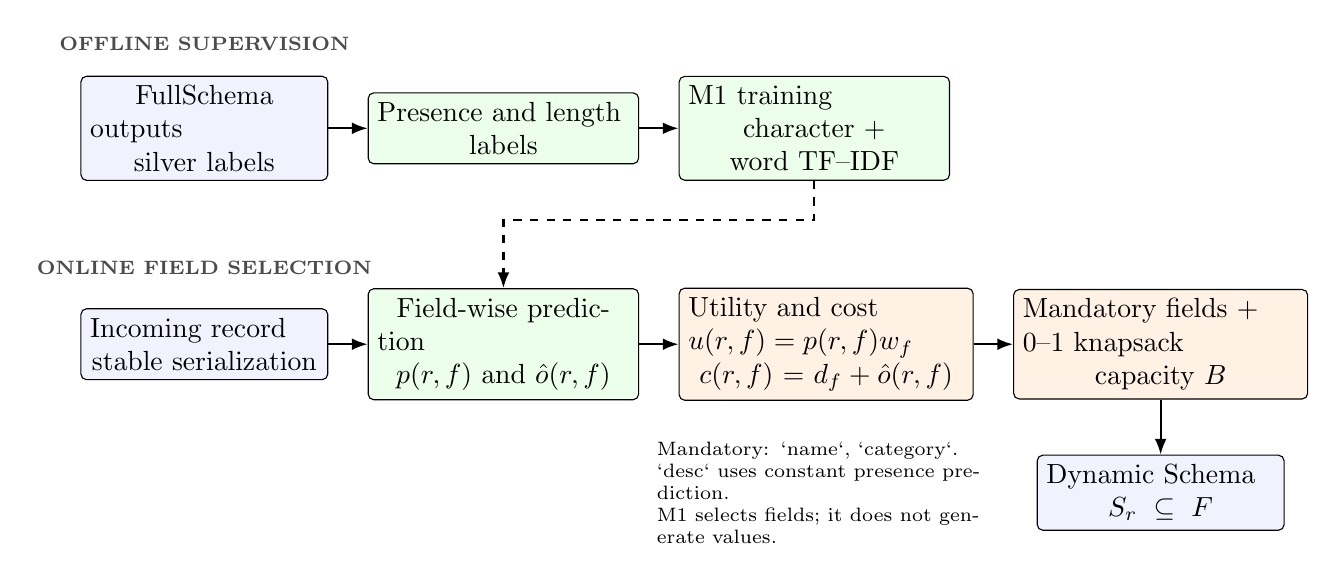
\begin{tikzpicture}[
  node distance=4mm and 5mm,
  box/.style={draw, rounded corners=2pt, align=center, minimum height=7mm,
    text width=29mm, fill=blue!5},
  model/.style={draw, rounded corners=2pt, align=center, minimum height=7mm,
    text width=32mm, fill=green!8},
  decision/.style={draw, rounded corners=2pt, align=center, minimum height=7mm,
    text width=35mm, fill=orange!10},
  note/.style={font=\scriptsize, align=left, text width=42mm},
  title/.style={font=\bfseries\scriptsize, text=black!70},
  arrow/.style={-{Latex[length=2mm]}, thick},
  dependency/.style={-{Latex[length=2mm]}, thick, dashed}
]
\node[title] (offline-title) {OFFLINE SUPERVISION};
\node[box, below=2mm of offline-title] (raw) {FullSchema outputs\newline silver labels};
\node[model, right=of raw] (labels) {Presence and length\newline labels};
\node[model, right=of labels] (train) {M1 training\newline character + word TF--IDF};
\draw[arrow] (raw) -- (labels);
\draw[arrow] (labels) -- (train);

\node[title, below=9mm of raw] (online-title) {ONLINE FIELD SELECTION};
\node[box, below=3mm of online-title] (record) {Incoming record\newline stable serialization};
\node[model, right=of record] (predict) {Field-wise prediction\newline $p(r,f)$ and $\hat{o}(r,f)$};
\node[decision, right=of predict] (score) {Utility and cost\newline $u(r,f)=p(r,f)w_f$\newline $c(r,f)=d_f+\hat{o}(r,f)$};
\node[decision, right=of score] (select) {Mandatory fields +\newline 0--1 knapsack\newline capacity $B$};
\node[box, below=7mm of select] (schema) {Dynamic Schema\newline $S_r\subseteq F$};
\node[note, left=of schema] (constraints) {Mandatory: `name`, `category`.\newline `desc` uses constant presence prediction.\newline M1 selects fields; it does not generate values.};
\draw[dependency] (train.south) -- ++(0,-5mm) -| (predict.north);
\draw[arrow] (record) -- (predict);
\draw[arrow] (predict) -- (score);
\draw[arrow] (score) -- (select);
\draw[arrow] (select) -- (schema);
\end{tikzpicture}%
}
\caption{M1-based dynamic field selection. FullSchema outputs provide model-assisted silver supervision offline. Online, the serialized record yields field-presence and output-length estimates, which are combined with auditable field weights and estimated costs under mandatory-field constraints to construct the record-level Schema. M1 selects fields only; actual values and API tokens are produced and measured downstream.}
\label{fig:m1-selection}
\end{figure}

\section{Experiments}
\subsection{Experimental Setup}
\subsubsection{Experimental Strategies}

Table~\ref{tab:strategies} distinguishes full-Schema, Prompt-only, dynamic-budget, and external-retrieval strategies.

\begin{table}[htbp]
\centering\scriptsize\renewcommand{\arraystretch}{0.88}
\caption{Inputs, selection mechanisms, and comparison roles of extraction strategies.}
\label{tab:strategies}
\resizebox{\linewidth}{!}{%
\begin{tabular}{>{\raggedright\arraybackslash}p{2.2cm}>{\raggedright\arraybackslash}p{3.3cm}>{\raggedright\arraybackslash}p{5.5cm}>{\raggedright\arraybackslash}p{3.4cm}}
\toprule
Strategy & Input fields & Field-selection or prompt mechanism & Comparison role\\
\midrule
`full` & All 18 fields & No pruning; base extraction prompt & Full-Schema baseline\\
`prompt-null` & All 18 fields & Output `null` without reliable evidence & Strict prompt-only baseline\\
`prompt-omit` & All 18 fields & Permit omitted fields without reliable evidence & Prompt-only output control\\
`budget-200/400` & Record-level field subset & \method{} prediction followed by a capacity-specific 0--1 knapsack & Dynamic strategy\\
`lambda` & Record-level field subset & \method{} prediction followed by a net-utility threshold & No-hard-budget control\\
`SchemaRAG k=10/15` & Top-$k$ field subset & Cosine ranking of query and field vectors & SchemaRAG-inspired efficiency reference\\
\bottomrule
\end{tabular}%
}
\end{table}

`budget-200/400` retains mandatory fields and solves a 0--1 knapsack; the no-hard-budget control uses $u(r,f)-0.003c(r,f)$. The main experiment has three repetitions of `full`, `budget-200`, and \schemarag{} $k=10$; other online strategies run once, and offline diagnostics are supplementary.

Estimated field costs are used only for pre-call decisions:
\begin{equation}
 \widehat{C}_{field}(r,f)=C_{schema}(f)+\widehat{C}_{output}(r,f).
\end{equation}
Here $C_{schema}(f)$ counts the field name and definition in `cl100k_base` tokens, and $\widehat{C}_{output}(r,f)$ is \method{}'s non-negative, truncated prediction of output length. This is not the actual API cost. The API records `input_tokens`, `output_tokens`, and `total_tokens` after the call, including retry overhead. Raw-record input and the fixed Prompt are usually sent regardless of field selection; they are excluded from the field-combination budget but included in online LLM token statistics.

\subsubsection{External Embedding-Based SchemaRAG Adaptation}

\schemarag{} is implemented as a SchemaRAG-inspired semantic field-selection reference for the same downstream LLM extraction pipeline. It does not use \method{} predictions or budget knapsack selection; instead, it ranks candidate fields by semantic similarity between the record and field descriptions. The candidate Schema in this study contains 18 fields, so this comparison evaluates field-load reduction in a compact JSON extraction setting rather than the large-Schema regime targeted by the original work.

\paragraph{Retrieval Representation and Field Ranking.}

Field-name and field-definition vectors are weighted 0.5/0.5 and normalized. The serialized JSON record and a fixed instruction form the single online query, and Top-10/15 fields are selected by cosine similarity. Thus, $k$ denotes the final number of retained fields here, corresponding to 55.6\% or 83.3\% of the 18-field candidate Schema. The original work instead targets schemas with hundreds to thousands of rows and uses $k$ for the number of examined embeddings; its reported scale and $k$ are therefore not directly comparable with ours. This adaptation uses only field-name and field-definition retrieval: it does not include the original method's optional example retrieval, in-context examples, text segmentation, or reranking. Field vectors are cached by configuration hash, while query embedding is included in pipeline time. Across three runs, the query-embedding stage averaged 129.30 ms and the Schema-vector stage 4.07 ms. The adaptation used Qwen3-Embedding-0.6B~\cite{zhang2025qwen3embedding}, batch size 32, a 60-s timeout, and 1024-dimensional vectors. It is therefore used as an external efficiency reference for token, latency, and extraction-behavior trade-offs, not as a complete reproduction of the original implementation. The embedding service does not return usage information, and its token consumption and server-side version cannot be reconstructed from the local archive.

\subsubsection{Online Execution and Metric Implementation}

The implementation is a single-process asynchronous bounded pipeline with a Producer, multiple Consumers, and a bounded queue. The concurrency `c` sets the number of Consumers and queue capacity `q` the queue size; a full queue blocks the Producer and creates backpressure. Tasks are built incrementally in input order, support checkpointed resumption by method and configuration hash, and failed tasks retain their error state after at most two retries.

We define makespan as the interval $t_{finish}-t_{start}$ and effective throughput as $N_{success}$ divided by makespan. The `pipeline_ms` interval covers online record reading, field prediction and selection, Prompt construction, enqueueing, LLM or embedding requests, retries, and result writing; each task stores Prompt, Schema, selector and method configuration hashes, selected fields, predicted and actual tokens, planning or retrieval time, latency, queue waiting, and error state.

The measured interval excludes startup-sample generation, silver-label construction, offline training, and model or vectorizer loading. System results are online inference results, not full-lifecycle costs; `budget-200` is an intermediate operating point, not a 200-token limit or globally optimal budget. This remains single-process, with no cross-process or cross-node scheduling.

\subsubsection{Evaluation Reference and Metrics}

Let $G_r$ be the non-empty fields in the model-assisted evaluation reference and $S_r$ the selected set. Unlike the `artifact_extract` silver labels used to train M1, this reference was generated at temperature 0 using only the raw record, with JSON null required when evidence was unreliable; it is not a human factual Gold. We define coverage as $\mathrm{Cov}(r)=|S_r\cap G_r|/|G_r|$ and omission as $\mathrm{Miss}(r)=1-\mathrm{Cov}(r)$. This metric measures field entry into the target Schema, not downstream output or factual correctness. The reference contains 500 records; the 476 records reported here are the success intersection of all eight historical methods. `full` and `budget-200` succeeded on all 500, and the remaining 24 were excluded because `prompt-omit` failed.

\subsubsection{Development-Distribution Workload and Conditions}

The performance workload contains 2,000 records from training and validation sets and does not overlap the test set, but overlaps \method{}'s development distribution and threshold calibration and is therefore not an independent generalization test. Samples were divided into five equal-frequency strata by raw-record byte length, with 400 records randomly drawn from each using seed 20260904. The main experiment compares `full`, \method{} `budget-200`, and \schemarag{} $k=10$, using 16 Consumers and a bounded queue of capacity 16, with three repetitions each. Other strategies were used only for implementation definitions or supplementary diagnostics.

\subsection{Experimental Results}
\subsubsection{Field-Selection Completeness}

\begin{table}[htbp]\centering\small
\caption{Field-selection completeness on the 476-record shared-success subset of 500 model-assisted evaluation-reference records.}\label{tab:coverage}
\begin{tabular}{@{}lccc@{}}\toprule
Method & Records & Reference-field coverage & Selection omission rate\\\midrule
full & 476 & 1.0000 & 0.00\%\\
budget-200 & 476 & 0.8303 & 16.97\%\\\bottomrule
\end{tabular}\end{table}

The zero omission of `full` follows from sending every candidate field and does not imply factual correctness. `budget-200` retains 83.03\% of non-empty reference fields, with 16.97\% omitted at selection. This is a measurable load--completeness trade-off, not lossless pruning. The 476-record quality set differs from the 2,000-record performance workload, so we make no cross-batch significance inference.

On the same 476-record shared-success subset, we further compare six internal Schema strategies in Table~\ref{tab:eight}. These metrics are computed against the model-assisted evaluation reference set and describe the relationship among field retention, output behavior, and tokens; they are not independent evidence of factual quality or global optimality.

\begin{table}[htbp]
\centering
\scriptsize
\setlength{\tabcolsep}{2pt}
\caption{Comparison of six internal methods on the 476-record shared-success subset of 500 model-assisted evaluation-reference records.}
\label{tab:eight}
\resizebox{\linewidth}{!}{%
\begin{tabular}{lccccc}
\toprule
Method & Macro-F1 & Micro-F1 & Exact Recall & Coverage & Total tokens\\
\midrule
full & .7623 & .7410 & .6528 & 1.0000 & 539.83\\
prompt-null & .6215 & .5871 & .6557 & 1.0000 & 548.01\\
prompt-omit & .7475 & .7386 & .6078 & 1.0000 & 487.10\\
budget-200 & .7759 & .7780 & .6213 & .8303 & 381.49\\
budget-400 & .7736 & .7638 & .6606 & .9763 & 486.32\\
lambda=0.003 & .7822 & .7816 & .6407 & .9606 & 441.28\\
\bottomrule
\end{tabular}%
}
\end{table}

Table~\ref{tab:eight} shows that the full field set is not a quality ceiling, while prompt constraints alone do not eliminate false positives from extra fields. Increasing the budget does not guarantee monotonically improving F1: `budget-400` increases Coverage but also increases token use. We therefore treat `budget-200` as an engineering compromise under the current data and service conditions, rather than a global optimum in quality or budget.

\subsubsection{Selection Mechanisms and Weight-Sensitivity Diagnostics}

To separate the effect of reducing the number of fields from that of a particular ranking mechanism, we compare selection strategies on 500 frozen model-assisted evaluation-reference records using five \method{} training seeds under the same mandatory fields and budget. Table~\ref{tab:selection-ablation} reports reference non-empty-field coverage. This is a selection-stage metric, and predicted tokens are selector estimates; neither represents online API usage or factual correctness.

\begin{table}[htbp]\centering\scriptsize\setlength{\tabcolsep}{3pt}
\caption{Selection-stage reference-field coverage (\%) on 500 frozen model-assisted reference records.}\label{tab:selection-ablation}
\begin{tabular}{@{}crrrrrr@{}}\toprule
Budget & Weighted & Equal & Frequency & \method{} Top-$k$ & Static Top-$k$ & Random Top-$k$\\\midrule
200 & 57.94 & 61.23 & 60.88 & 65.55 & 65.55 & 46.03\\
400 & 94.22 & 93.16 & 95.06 & 94.68 & 95.97 & 60.86\\\bottomrule
\end{tabular}\end{table}

Random Top-$k$ is substantially lower at both budgets, indicating that arbitrary field reduction does not preserve reference fields equally well. The current hand-weighted strategy is not consistently better than equal weighting, training frequency, or simple Top-$k$: after $\pm20\%$ multiplicative perturbations, coverage at budgets 200/400 was 57.51\% and 94.00\%, close to the original 57.94\% and 94.22\%, so no catastrophic decline occurred but unique or optimal weights are not established. The five-seed sensitivity intervals used the Student-$t$ distribution. Perturbation results summarize $5\times20$ preset combinations, and random Top-$k$ uses 20 fixed random seeds per model; neither represents 100 independent model trainings.

\subsubsection{Main Online Comparison}

\begin{table}[htbp]\centering\scriptsize\setlength{\tabcolsep}{2pt}
\caption{Online-system results on the 2,000-record development-distribution workload.}\label{tab:system}
\begin{tabular}{@{}lccccc@{}}\toprule
Method & $N_{success}/N_{total}$ & Makespan (s) & Effective throughput & Total tokens & P99 (ms)\\\midrule
full & 2000/2000 & 220.82 & 9.06 & 1,709,102 & 3,601\\
budget-200 & 2000/2000 & 113.64 & 17.61 & 1,069,254 & 1,308\\
SchemaRAG $k=10$ & 1998/2000 & 399.68 & 5.03 & 1,230,411 & 19,886\\\bottomrule
\end{tabular}\end{table}

\begin{figure}[htbp]\centering
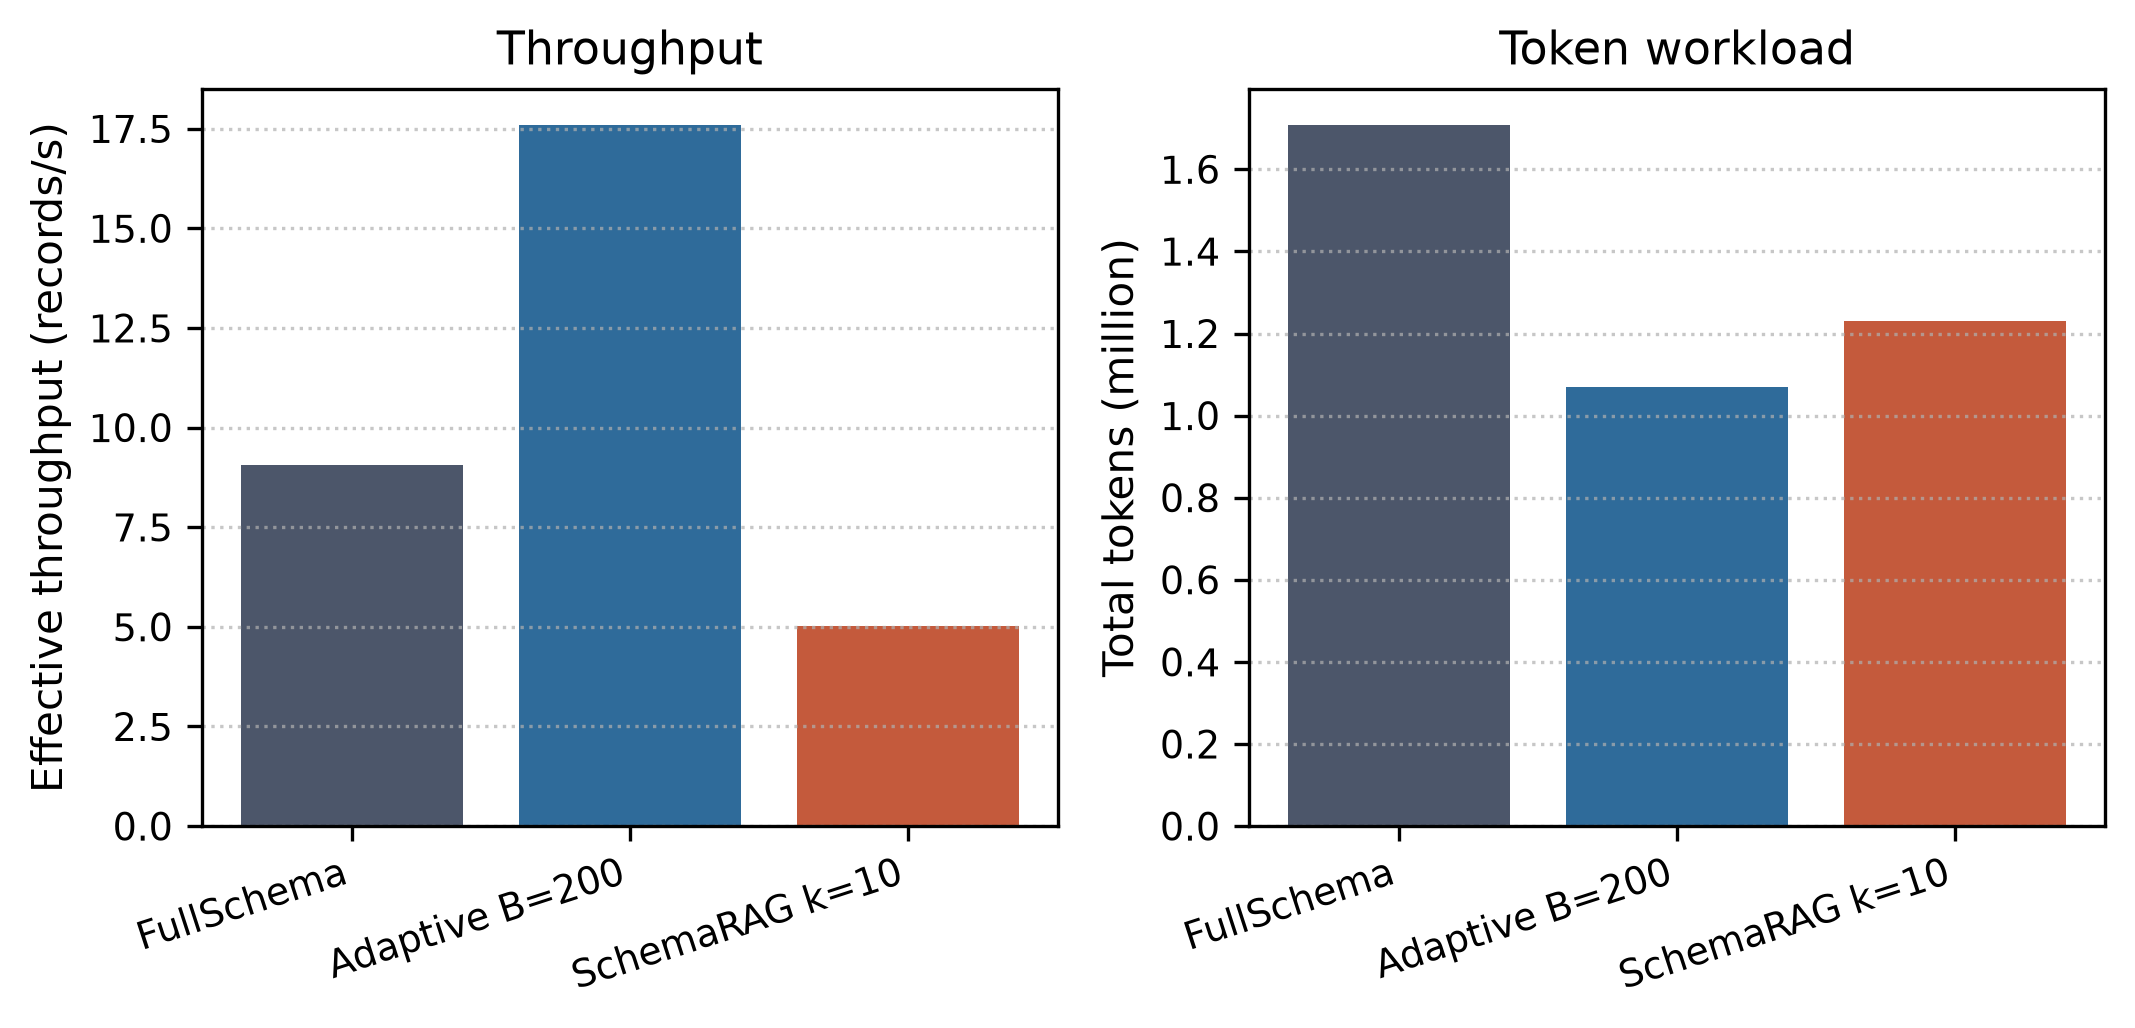
\includegraphics[width=.47\linewidth]{main_throughput_and_tokens.png}\hfill
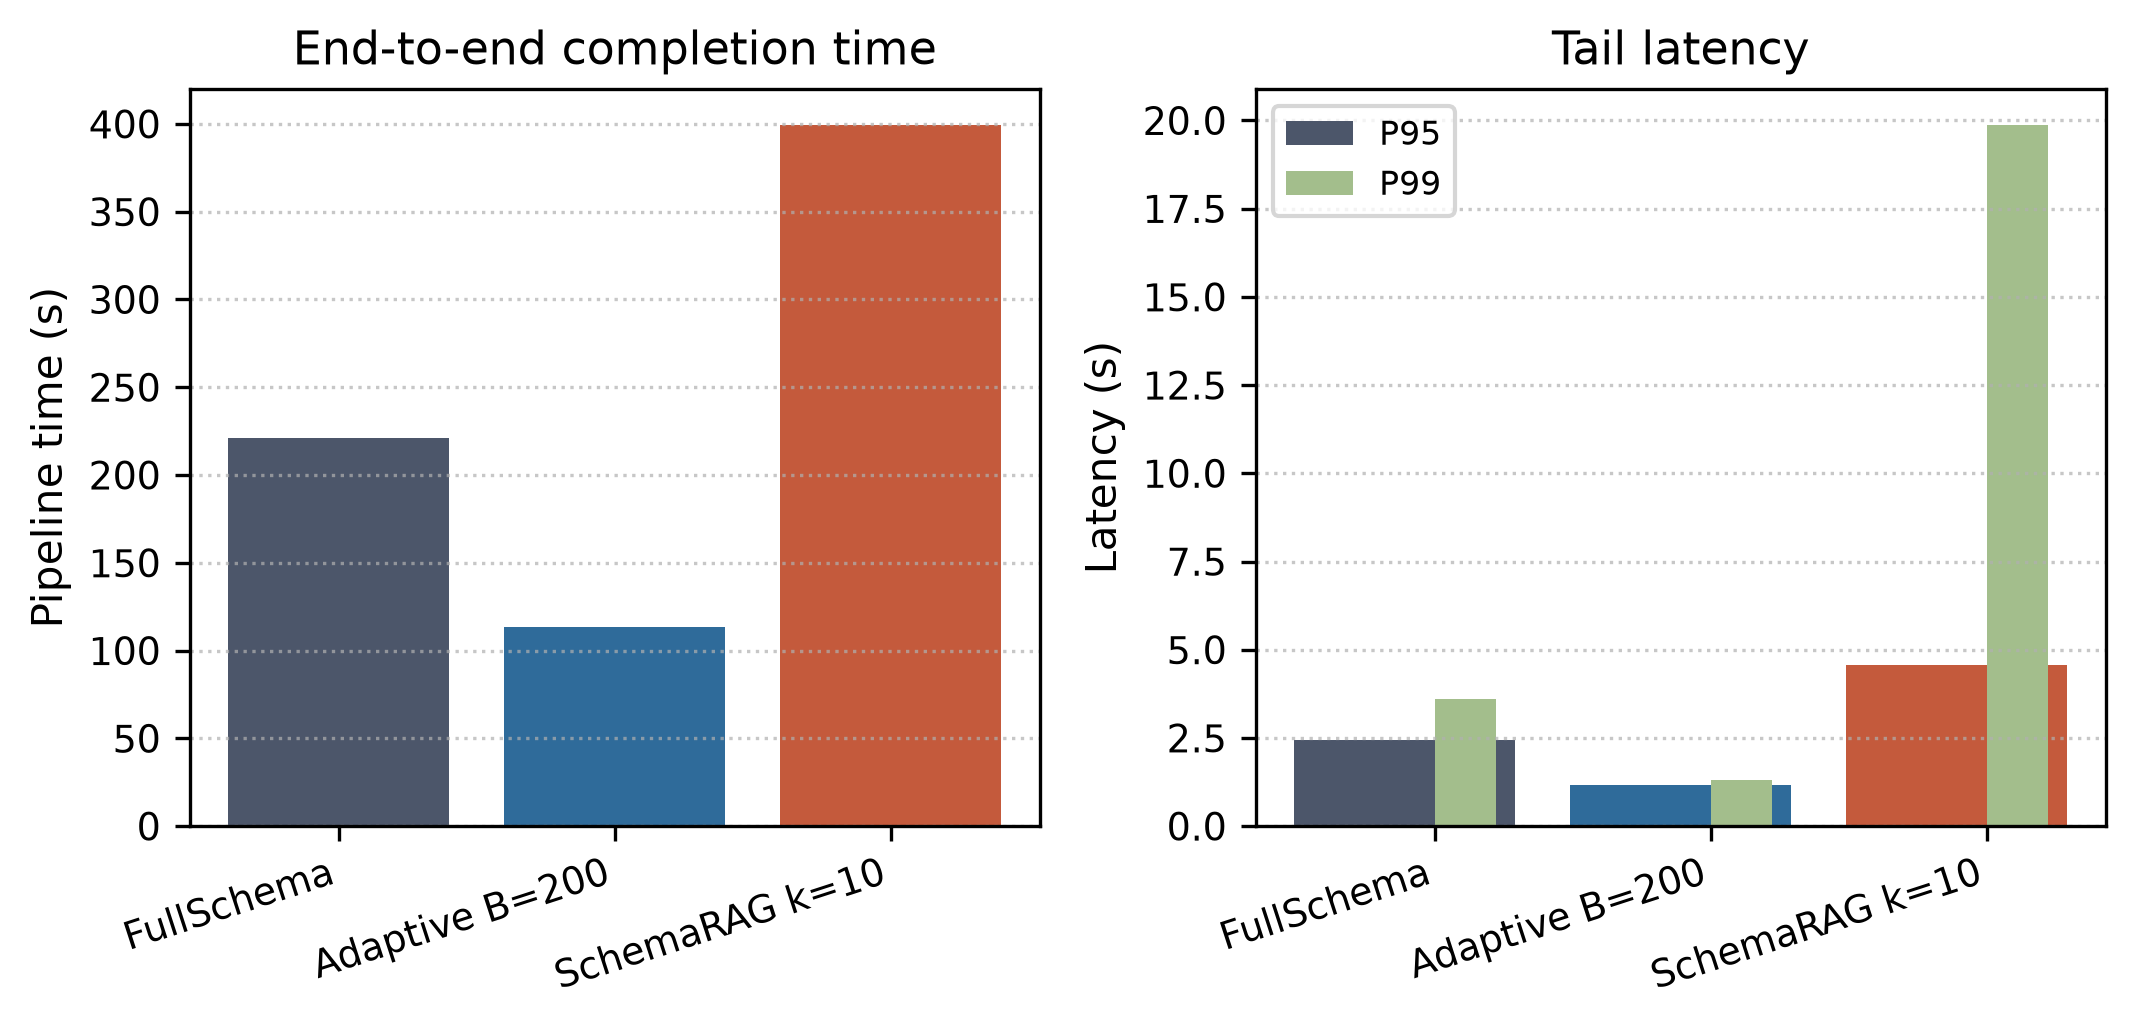
\includegraphics[width=.47\linewidth]{main_time_and_tail_latency.png}
\caption{Main online comparison on the 2,000-record development-distribution workload, showing effective throughput, LLM token workload, makespan, and P99 latency for the three-run main experiment; the comparison is limited to the stated model service and concurrency configuration.}\label{fig:system-main}
\end{figure}

\begin{sloppypar}
Across three repetitions, `budget-200` used less time and fewer tokens and achieved higher throughput than `full`. Their 95\% $t$ intervals for time were 106.94--120.35 s and 216.85--224.80 s, respectively. Mean P95/P99 latencies were 2,438/3,601, 1,161/1,308, and 4,572/19,886 ms for `full`, `budget-200`, and \schemarag{}, respectively. Across three runs, each method processed 6,000 tasks: `full` and `budget-200` had no failures or retries; \schemarag{} had six final failures and 12 retries, all caused by output keys outside the target set. `Total tokens` includes LLM input, output, and retries but excludes embedding; mean input/output tokens were 1,399,176/309,926, 939,791/129,463, and 1,019,842/210,569 for the same three methods, respectively.
\end{sloppypar}

\subsubsection{Budget Response and Supplementary Online Baselines}

We scanned nine budget settings once under the same 2,000-record workload and $c=16,q=16$. The field ratio is selected fields divided by the 18 candidate fields, not reference-field coverage; tokens are the sum of actual LLM input and output, and the budget remains only a selection-stage capacity.

\begin{table}[htbp]\centering\scriptsize\setlength{\tabcolsep}{3pt}
\caption{Single-run online budget response on the 2,000-record frozen workload.}\label{tab:budget-response}
\begin{tabular}{@{}rrrrrr@{}}\toprule
Budget & LLM Token/record & Fields/record & Fields/18 (\%) & P99 (ms) & Success (\%)\\\midrule
60 & 326.7 & 2.80 & 15.5 & 1240 & 100.00\\
100 & 404.0 & 4.15 & 23.1 & 993 & 100.00\\
150 & 482.4 & 5.90 & 32.8 & 1186 & 99.95\\
200 & 534.6 & 7.52 & 41.8 & 1445 & 100.00\\
300 & 627.4 & 10.13 & 56.3 & 1706 & 100.00\\
400 & 730.7 & 13.73 & 76.3 & 2818 & 100.00\\
600 & 856.1 & 18.00 & 100.0 & 3883 & 100.00\\
800 & 857.6 & 18.00 & 100.0 & 3870 & 100.00\\
1200 & 858.0 & 18.00 & 100.0 & 3915 & 100.00\\\bottomrule
\end{tabular}\end{table}

\begin{figure}[htbp]\centering
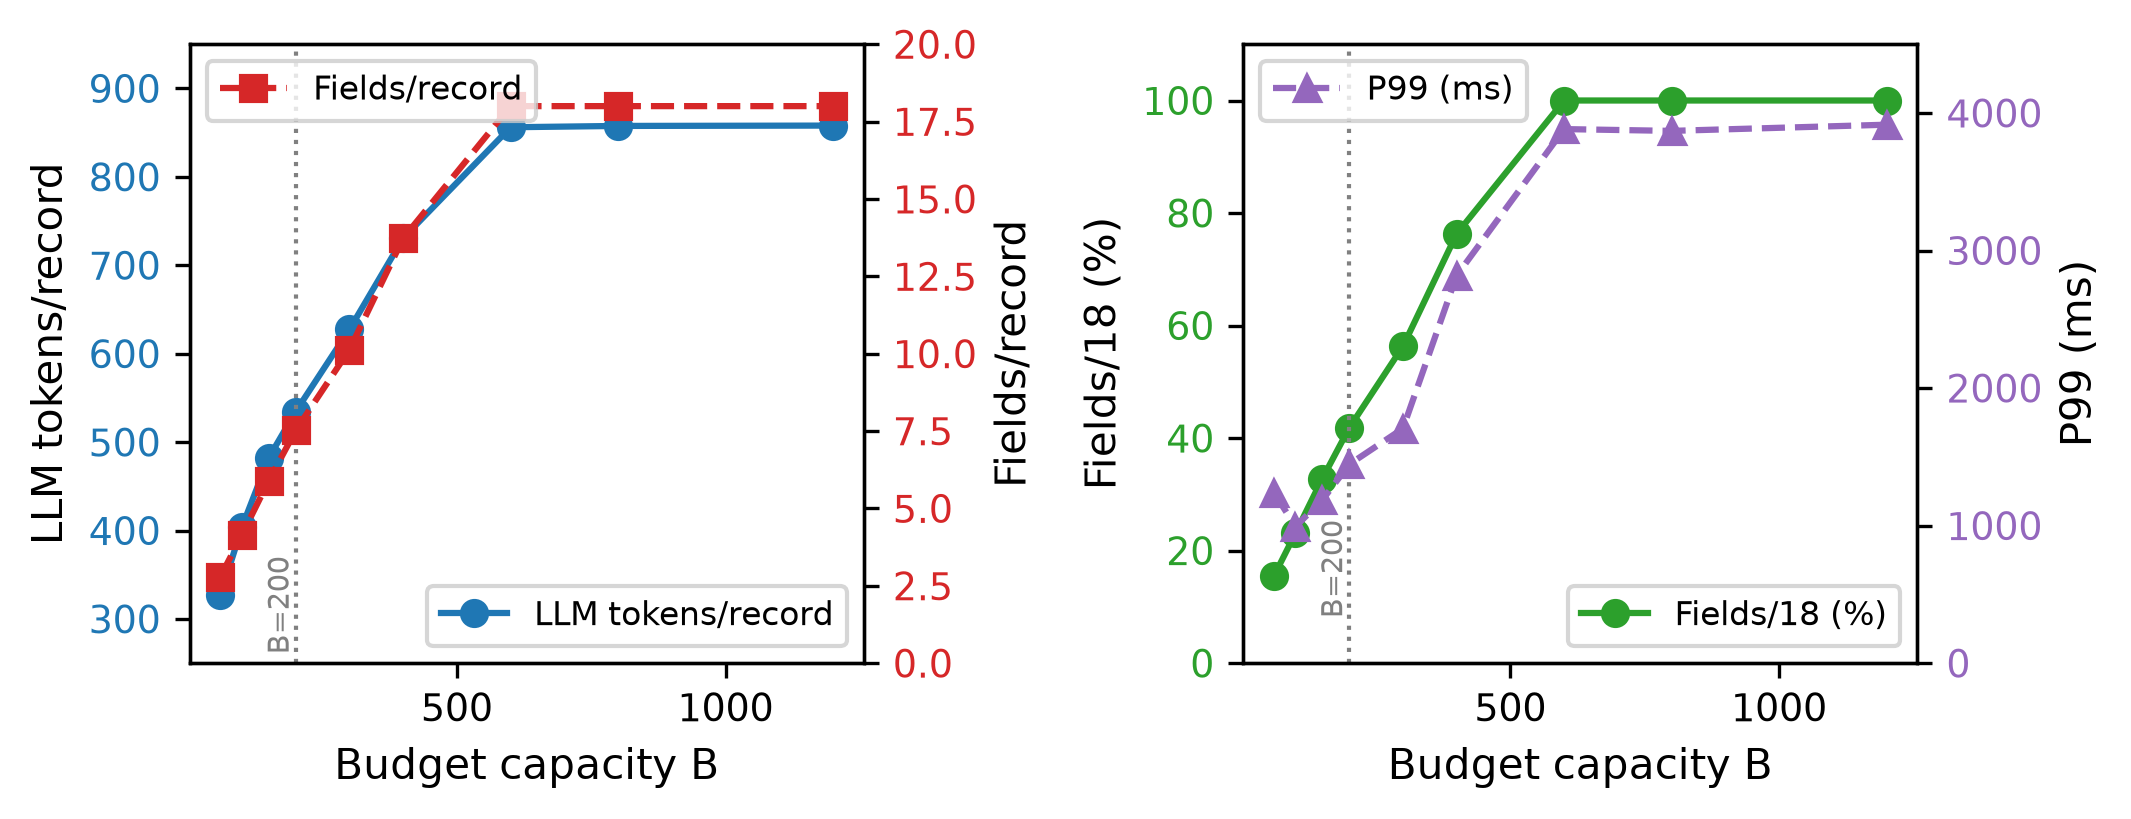
\includegraphics[width=.72\linewidth]{budget_response.png}
\caption{Online budget response on the 2,000-record frozen workload (single run each). Left: LLM tokens/record and fields/record; right: Fields/18 (\%) and P99; the dashed line marks $B=200$.}\label{fig:budget-response}
\end{figure}

Actual tokens and field counts generally increase with the budget and saturate near 600 units, when all 18 fields are selected. `budget-200` is therefore a low-to-intermediate operating point, not a global optimum; its 41.8\% field ratio does not measure reference-field completeness. The 60--400 range supports choosing a load subject to acceptable omission, tokens, tail latency, and success rate.

In a single supplementary baseline run, LLM tokens per record for $\lambda=0.003$, prompt-omit, and prompt-null were 625.5/823.2/892.6, and P99 values were 3575/2542/3903 ms. Prompt-only controls still used all fields, indicating that token reduction mainly comes from reducing the number of fields; \method{}'s ranking advantage has not been established. Random/frequency Top-$k$ online results remain unavailable.

\subsubsection{Directional Endpoint Validation}

To separate the directional effects of concurrency and queue capacity, we scanned 500 records: with $c=16$ fixed, $q\in\{4,8,16,32,64\}$; with $q=16$ fixed, $c\in\{1,2,4,8,16,32\}$. Every point used `budget-200` and achieved 500/500 successes; the first $q=64$ run submitted only 182 records owing to a shell timeout and was replaced by a clean rerun of all 500. With $c=16$ fixed, throughput was 21.04, 21.31, 21.54, 20.20, and 21.01 records/s for the five queue sizes, while queue-wait P99 was 578, 758, 997, 1,908, and 3,265 ms. With $q=16$ fixed, throughput was 1.67, 3.34, 6.52, 11.80, 21.54, and 30.19 records/s for the six concurrency levels.

With fixed $c$, increasing $q$ mainly raises the queue-wait tail without a stable throughput gain. With fixed $q$, increasing $c$ improves throughput but high concurrency raises tail latency. This scan remains single-process and cannot establish production-scale scalability; it also shows that optimization should monitor time, success rate, and tail latency in addition to token minimization.

\subsubsection{Initialization-Cost Boundary}

Isolated training on 100 \method{} samples took $737.13\pm43.69$ ms; the model occupied 3.36 MB and cold loading took $178.26\pm14.43$ ms. A local planning batch of 100 records took 366.63 ms, while the independent stage measurement was $3.09\pm0.16$ ms per record and complete planning plus prediction and Prompt construction took approximately 6.2 ms per record; these measurements use different scopes. Based on the measured one-time startup cost of 915.39 ms and the online difference, the budget--full time break-even is approximately 17 records (Fig.~\ref{fig:init-cost}), while the token break-even is zero. \schemarag{} did not obtain a time benefit in the current range. This estimate excludes startup-sample generation, environment startup, and cold-cache effects and is not a monetary-cost or full-lifecycle audit.

\begin{figure}[htbp]\centering
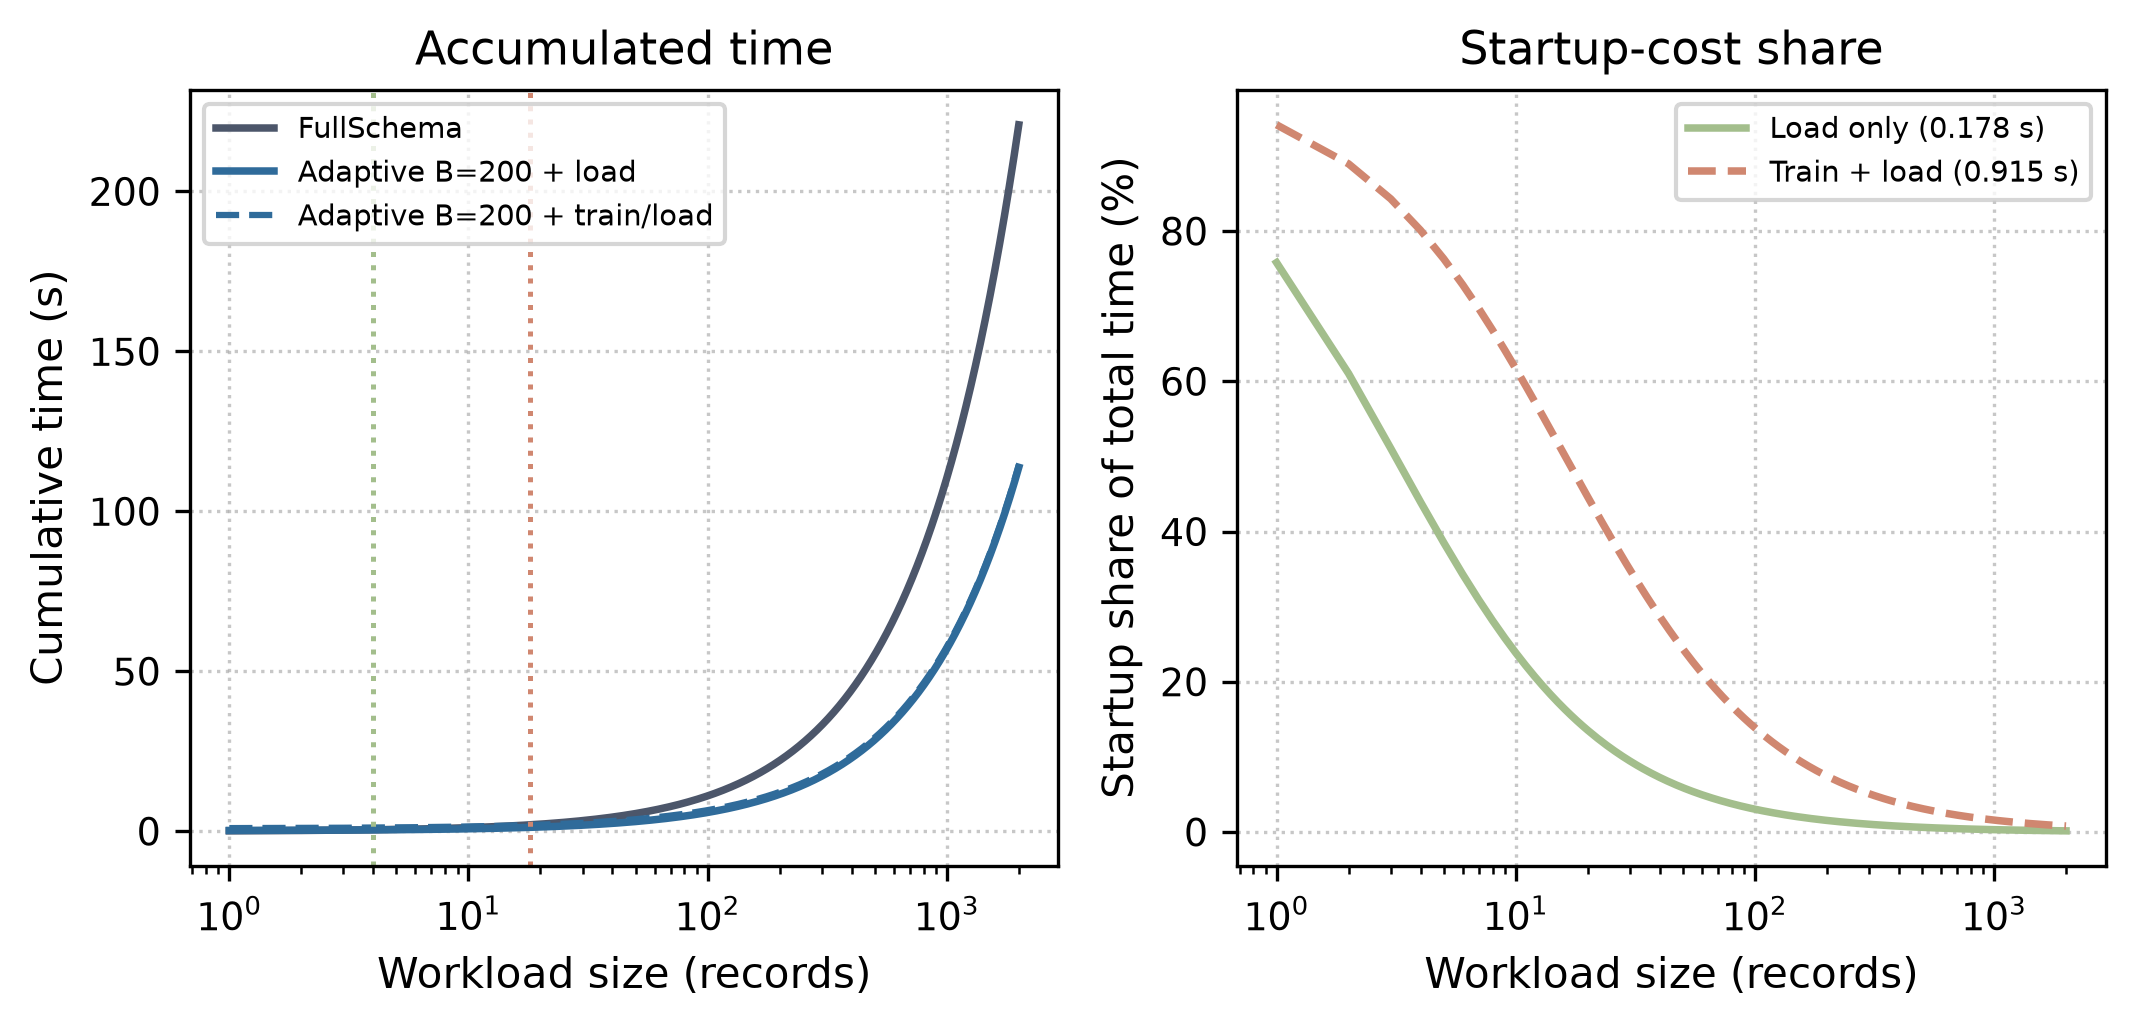
\includegraphics[width=.72\linewidth]{initialization_cost_sensitivity.png}
\caption{Initialization-cost sensitivity and the budget--full time break-even. The curve marks the one-time startup cost and the point where the dynamic-selection overhead is recovered.}\label{fig:init-cost}
\end{figure}

\subsection{Discussion}

 Under the current single-process pipeline and service configuration, `budget-200` coincided with fewer tokens, a shorter makespan, and higher effective throughput. The \schemarag{} comparison shows that retrieval overhead can offset savings from reducing field load, so load shaping should be evaluated through field-selection completeness, end-to-end time, throughput, success rate, and tail latency.

 Explicitly limiting Schema load within an auditable budget changes the online cost profile, but does not establish optimal ranking, field importance, or factual-quality equivalence to `full`. The budget scan supports capacity-based load control and eventual saturation, while the approximate field-count baseline and offline ablation provide no stable advantage for the current \method{} weighted knapsack. Thus, the supported mechanism is field-load control under a budget, not ranking optimality.

  The 476-record omission analysis uses a non-human reference, and the workload comes from the development distribution. The \schemarag{} result is an efficiency reference for the present 18-field setting and should not be extrapolated to the large-Schema regime targeted by the original work. The system and concurrency scans are single-process, exclude lifecycle costs, and include supplementary points run only once. Human-validated evaluation on an unseen workload, with near-duplicate isolation and multi-process scheduling, remains necessary.

 A plausible applicability condition is that training and deployment records share similar field semantics, textual patterns, and information distributions. The selector may exploit stable associations between raw-record cues and candidate-field presence, but this interpretation was not separately tested; substantial cross-template or cross-source shifts remain unassessed.

\section{Conclusion}

\begin{sloppypar}
\setlength{\emergencystretch}{4em}
We proposed and evaluated a budget-aware dynamic Schema-selection pipeline trained from \full{} model-assisted silver labels. With the current model, a single-process Runner, $c=16,q=16$, and a 2,000-record development-distribution workload, \method{} `budget-200` coincided with fewer tokens, shorter pipeline time, and higher effective throughput. Its reference-field coverage on the paired quality set was 83.03\%, with 16.97\% omitted at selection.
\end{sloppypar}

The results demonstrate an engineering trade-off between efficiency and field-selection completeness, rather than lossless pruning. The budget curve supports capacity-based load control, while the approximate field-count baseline and offline ablation indicate no stable optimality for the current ranking or hand-designed weights. The reference does not verify factual field-value quality, and the results do not establish independent generalization or production-scale scalability.

\bibliographystyle{splncs04}
\bibliography{references}
\end{document}
